\documentclass{zkdl-presentation-template}

\title[Bulletproofs: inner-product argument]{\textbf{Bulletproofs: applications}}
\author{Distributed Lab}
\date{July 31, 2025}
\homepage{zkdl-camp.github.io}
\github{ZKDL-Camp}

\begin{document}

\frame {
    \tikz [remember picture,overlay]
    \node at
    ([yshift=1.5cm,xshift=-1.5cm]current page.south east)
%or: (current page.center)
        {
\includegraphics[width=60pt]{images/logo.png}};

    \titlepage
}

\begin{frame}{Plan}
    \tableofcontents
\end{frame}

\section{Introduction}

\begin{frame}{Inner-product argument: illustration}
    \begin{figure}[h!]
        \centering
        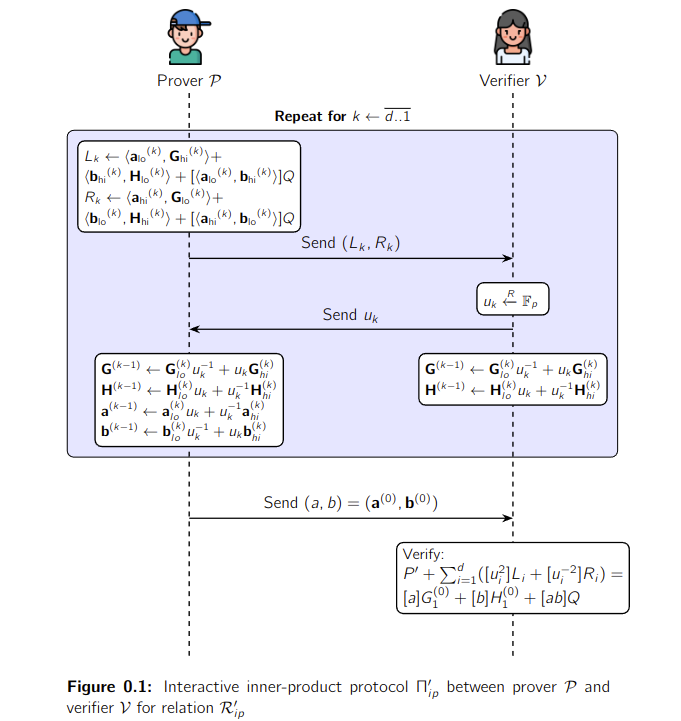
\includegraphics[width=0.8\textwidth]{images/lecture_17/ipa.png}
        \label{fig:ipa}
    \end{figure}
\end{frame}

\begin{frame}{Recap: inner-product argument}
    \begin{itemize}
        \item \textbf{Goal:} Prove $\langle \mathbf{a}, \mathbf{b} \rangle = c$ with logarithmic proof size
        \item Commitment: $P' = \langle \mathbf{a}, \mathbf{G} \rangle + \langle \mathbf{b}, \mathbf{H} \rangle + [\langle \mathbf{a,b} \rangle]Q$
        \item Protocol recursively compresses vectors, sending $L_k, R_k$ at each step
        \item Final check: $P' + \sum ([u_i^2]L_i + [u_i^{-2}]R_i) = [a]G + [b]H + [ab]Q$
    \end{itemize}
    \begin{alertblock}{Key property}
        Proof size is $2\log_2 n$ group elements $+$ $2$ scalars. Protocol is \textit{knowledge sound} and \textit{perfect complete} but not \textit{zero-knowledge}.
    \end{alertblock}
    \begin{block}{Idea}
        We could provide \textit{zero-knowledge} directly to \textit{inner-product argument} construction or use \textbf{zk-mul} protocol for outer construction.
    \end{block}
\end{frame}

\begin{frame}{Recap: zkmul}
    Consider relation $R_{mul} = \{ (\bot; l(x), r(x), t(x)) \vert t(x) = l(x)r(x) \}$ where $l(x) = a + s_L x, r(x) = b + s_R x, t(x) = l(x)r(x)$. Protocol \textbf{zk-mul} is defined as follows:

    \begin{itemize}
        \item Prover computes and sends to $\mathcal{V}$ commitments to $l(x), r(x), t(x)$:
            \begin{align*}
                A &= [a]G + [b]H + [\alpha]B & T_0 &= [ab]G + [\tau_0]B\\
                S &= [s_L]G + [s_R]H + [\beta]B &T_1 &= [s_L + s_R]G + [\tau_1]B\\
                &&T_2 &= [s_Ls_R]G + [\tau_2]B
            \end{align*}
            \item Verifier draws random challenge $u \in \mathbb{F}_p$ and sends it to prover
            \item Prover evaluates and sends to Verifier $(l_u, r_u, t_u, \alpha_u, \tau_u)$: 
            \begin{align*}
                l_u =l(u), r_u = r(u), t_u = l_u \cdot r_u, 
                \alpha_u = \alpha + \beta u, \tau_u = \tau_0 + \tau_1 u + \tau_2 u^2
            \end{align*}
            \item Verifier checks: $A + [u]S \stackrel{?}{=} [l_u]G + [r_u]H + [\alpha_u]B$, $[t_u]G + [\tau_u]B \stackrel{?}{=} T_0 + [u]T_1 + [u^2]T_2$, $t_u \stackrel{?}{=} l_u r_u$
    \end{itemize}
\end{frame}

\section{IPA polynomial commitment scheme}

\begin{frame}{Recap: Polynomial commitments}
    \begin{itemize}
        \item \textbf{Polynomial commitment scheme} $$\mathcal{C} = (\mathsf{Setup}, \mathsf{Commit}, \mathsf{Open}, \mathsf{VerifyOpen})$$ allows to commit to a polynomial $f(x) = \sum_{i=0}^{n-1} a_i x^i$ and prove its evaluation at some point.
        \item \textbf{Applications:} SNARKs compiled with IOP + polynomial commitment scheme framework (e.g., Halo, Nova, Spartan, Plonk)
        \item \textbf{Desirable properties:} sublinear size, efficient, no trusted setup
    \end{itemize}
    \begin{example}
        One famouos example is the \textbf{KZG} polynomial commitment scheme, which uses bilinear pairings and requires a trusted setup.
    \end{example}
\end{frame}

\begin{frame}{IPA polynomial commitment}
    Let $f(x) = \sum_{i=0}^{n-1} a_i x^i$ be a polynomial of degree $n-1=2^d-1$.
    
    The \textbf{non-hiding IPA polynomial commitment scheme} $\mathcal{C}_{ip} = (\mathsf{Setup, Commit, Open, VerifyOpen})$ is defined as follows:
    \begin{itemize}
        \item $\textcolor{teal}{\mathsf{Setup}}$ returns independent generators $\mathbf{G} = (G_1, \dots, G_n)$.
        \item $\textcolor{teal}{\mathsf{Commit}}$ returns $\mathsf{Com}(f) = \langle \mathbf{f}, \mathbf{G} \rangle$ where $\mathbf{f} = (a_0, \dots, a_{n-1})$
        \item $\textcolor{teal}{\mathsf{Open}}$ given evaluation point $u \in \mathbb{F}_p$ computes $\mathbf{u^n} = (1, u, u^2, \dots, u^{n-1})$,  obtains $f(u) = \langle \mathbf{f, u^n} \rangle$ and runs \textit{inner-product argument} $\Pi_{ip}$ non-interactively setting 
        $$\mathbf{a} = \mathbf{f}, \mathbf{b} = \mathbf{u^n}, P = \mathsf{Com}(f), c = f(u)$$ 
        to produce an evaluation proof $\pi_{ip}$
        \item $\textcolor{teal}{\mathsf{VerifyOpen}}$ given evaluation point $u \in \mathbb{F}_p$ and commitment $\mathsf{Com}(f)$ validates proof $\pi_{ip}$ running the non-interactive verifier $\mathcal{V}$ of \textit{inner-product} argument.
    \end{itemize}
\end{frame}

\section{Range proofs}

\begin{frame}{Range proofs: motivation}
    \begin{itemize}
        \item \textbf{Goal:} Prove $v \in [0, 2^n)$ without revealing $v$:
        $$\mathcal{R}_{rp} = \{ (G, B, V, n; v, \gamma) \vert V = [v]G + [\gamma]B, v \in [0, 2^n) \}$$
        \item \textbf{Applications:} Confidential transactions (e.g., Monero, Mimblewimble), other privacy-preserving protocols.
        \item \textbf{Idea}: Prove $v = \sum_{i=0}^{n-1} v_i 2^i$ and $\forall i \in 0..n-1: v_i \in \{0,1\}$
        \begin{block}{Naive approach}
            One could prove $v = \sum_{i=0}^{n-1} v_i 2^i$ and $\forall i \in 0..n-1: v_i \in \{0,1\}$ using $\Sigma$-protocols, but this would be inefficient due to linear proof.
        \end{block}
    \end{itemize}
\end{frame}

\begin{frame}{Compiling range proof into inner-product}
    Firstly, write $v$ in base-2 representation: $v = \sum_{i=0}^{\lfloor \log_2 v \rfloor} 2^i v_i$ and $\mathbf{a}_L = (v_0, v_1, \dots, v_{n-1})$ be the vector of bits padded with zeroes to length $n$, define $\mathbf{a}_R = \mathbf{a}_L - \mathbf{1}^n$ so the range validation that $v$ lays in $[0, 2^n)$ implies two checks:
    \begin{itemize}
        \item The following inner-product equality holds: $\langle \mathbf{a}_L, \mathbf{2}^n \rangle = v$
        \item Each bit $v_i$ must be either $0$ or $1$:
        \begin{align*}
        \mathbf{a}_L - \mathbf{a}_R - \mathbf{1}^n = \mathbf{0}^n \\
        \mathbf{a}_L \circ \mathbf{a}_R = \mathbf{0}^n
        \end{align*}
        \begin{example}
            Let $\mathbf{a}_L = (1, 0, 1, 0)$, $\mathbf{a}_R = (0, -1, 0, -1)$, then 
            $\mathbf{a}_L \circ \mathbf{a}_R = (0, 0, 0, 0)$
        \end{example}
    \end{itemize}
\end{frame}

\begin{frame}{Compiling range proof into inner-product}
    This two checks imply verification that some vector is zero vector, for that we use some challenge $y \in \mathbb{F}_p$ and check inner-product equalities $$\langle \mathbf{a}_L \circ \mathbf{a}_R, \mathbf{y}^n \rangle = 0 \text{ and } \langle \mathbf{a}_L - \mathbf{a}_R - \mathbf{1}^n, \mathbf{y}^n \rangle = 0$$
    This checks are sound because the prover doesn't know challenge $y$ in advance. So we must combine three inner-product checks:
    \begin{enumerate}
    \item $\langle \mathbf{a}_L, \mathbf{2}^n \rangle = v$
    \item $\langle \mathbf{a}_L, \mathbf{a}_R \circ \mathbf{y}^n \rangle = 0$
    \item $\langle \mathbf{a}_L - \mathbf{a}_R - \mathbf{1}^n, \mathbf{y}^n \rangle = 0$
    \end{enumerate}
    into one soundly summing up with powers of other challenge $z \in \mathbb{F}_p$:
    $$z^2 \cdot \langle \mathbf{a}_L, \mathbf{2}^n \rangle + z \cdot \langle \mathbf{a}_L - \mathbf{a}_R - \mathbf{1}^n, \mathbf{y}^n \rangle + \langle \mathbf{a}_L, \mathbf{a}_R \circ \mathbf{y}^n \rangle = z^2v$$
\end{frame}

\begin{frame}{Compiling range proof into inner-product}
    Using some dark linear algebra wizardry we could combine the three inner-product checks into a single one inner-product check:
    \begin{equation*}
        \langle \mathbf{a}_L - z \cdot \mathbf{1}^n, z^2 \cdot \mathbf{2}^n + z \cdot \mathbf{y}^n + \mathbf{a}_R \circ \mathbf{y}^n\rangle = z^2v + \delta(y,z)
    \end{equation*}
    Where $\delta(y,z)$ could easily be computed by verifier:
    $$\delta(y,z) = (z-z^2)\langle \mathbf{1}^n, \mathbf{y}^n \rangle - z^3 \langle \mathbf{1}^n, \mathbf{2}^n \rangle $$
    Now it's time to bring out \textbf{zk-mul} for inner-products! 
    
    Firstly, construct the blinding polynomials for $\mathbf{a}_L$ and $\mathbf{a}_R$:
    $$\mathbf{a}_L' \gets \mathbf{a}_L + \mathbf{s}_L x \quad \mathbf{a}_R' \gets \mathbf{a}_R + \mathbf{s}_R x$$
    Compute polynomials $\mathbf{l}(x) = \mathbf{l}_0 + \mathbf{l}_1 x, \quad \mathbf{r}(x) = \mathbf{r}_0 + \mathbf{r}_1 x$:
    \begin{align*}
        \mathbf{l}(x) &= \mathbf{a}_L' - z \cdot \mathbf{1}^n = (\mathbf{a}_L + \mathbf{s}_L x) - z \cdot \mathbf{1}^n = \textcolor{teal}{\mathbf{a}_L - z \cdot \mathbf{1}^n} + \mathbf{s}_L x\\
        \mathbf{r}(x) &= z^2 \cdot \mathbf{2}^n + z \cdot \mathbf{y}^n + \mathbf{a}_R' \circ \mathbf{y}^n = z^2 \cdot \mathbf{2}^n + z \cdot \mathbf{y}^n + (\mathbf{a}_R + \mathbf{s}_R x) \circ \mathbf{y}^n \\
        & = \textcolor{orange}{z^2 \cdot \mathbf{2}^n + z \cdot \mathbf{y}^n + \mathbf{a}_R \circ \mathbf{y}^n} + \mathbf{s}_R \circ \mathbf{y}^n x
    \end{align*}
\end{frame}

\begin{frame}{Compiling range proof into inner-product}
    $$t(x) = \langle \mathbf{l}(x), \mathbf{r}(x) \rangle = t_0 + t_1 x + t_2 x^2$$
    Now $\mathcal{P}$ needs to apply \textbf{zk-mul} for proving: $$t_0 =  \langle \textcolor{teal}{\mathbf{a}_L - z \cdot \mathbf{1}^n}, \textcolor{orange}{z^2 \cdot \mathbf{2}^n + z \cdot \mathbf{y}^n + \mathbf{a}_R \circ \mathbf{y}^n}\rangle = z^2v + \delta(y,z)$$ 
    \textbf{Note}: $\mathcal{V}$ could compute commitment $Com(t_0)$ using $V=Com(v)$
    \begin{alertblock}{Remark}
    We couldn't apply raw \textbf{zk-mul} as $\mathbf{l}_0$ depends on verifier-provided challenges, instead $\mathcal{P}$ firstly commits to $\mathbf{a}_L, \mathbf{a}_R$ and blinders $\mathbf{s}_L, \mathbf{s}_R$, obtaints challenges $y,z$ from $\mathcal{V}$ and computes rest of the commitments. 
    
    During verification phase $\mathcal{V}$ should adjust commitments to $\mathbf{l}(x), \mathbf{r}(x)$ by himself using homomorphic proterties of Pedersen commitment scheme.
    \end{alertblock}
\end{frame}

\begin{frame}{Range proofs: building the protocol}
    \begin{itemize}
        \item $\mathsf{Setup}$ returns independent generators $\mathbf{G}, \mathbf{H} \in \mathbb{G}^n$
        \item Prover does bit decomposition of $v$: $\mathbf{a}_L \gets \mathbf{v}, \mathbf{b_L} \gets \mathbf{a}_L - \mathbf{1}^n$, choses blinding terms $\mathbf{s}_L, \mathbf{s}_R \in \mathbb{F}_p^n, \alpha, \beta \in \mathbb{F}_p$, sends commitments:
            \begin{align*}
                A = \langle \mathbf{a}_L, \mathbf{G} \rangle + \langle \mathbf{b_L}, \mathbf{H} \rangle + [\alpha]B &&
                S = \langle \mathbf{s}_L, \mathbf{G} \rangle + \langle \mathbf{s}_R, \mathbf{H} \rangle + [\beta]B
            \end{align*}
        \item Verifier $\mathcal{V}$ samples challenges $y, z \xleftarrow{R} \mathbb{F}_p$ and sends them to $\mathcal{P}$
        \item Prover $\mathcal{P}$ reconstructs polynomials $\mathbf{l}(x), \mathbf{r}(x), \mathbf{t}(x)$:
            \begin{equation*}
                \begin{aligned}
                    \mathbf{l}(x) &= \mathbf{a}_L - z \cdot \mathbf{1}^n + \mathbf{s}_L x\\
                    \mathbf{r}(x) &= z^2 \cdot \mathbf{2}^n + z \cdot \mathbf{y}^n + \mathbf{a}_R \circ \mathbf{y}^n + \mathbf{s}_R \circ \mathbf{y}^n x\\
                    t(x) &= \langle \mathbf{l}(x), \mathbf{r}(x) \rangle = t_0 + t_1 x + t_2 x^2
                \end{aligned}
            \end{equation*}
            \begin{equation*}
                \begin{aligned}
                    t_0 &=  \langle \textcolor{teal}{\mathbf{a}_L - z \cdot \mathbf{1}^n}, \textcolor{orange}{z^2 \cdot \mathbf{2}^n + z \cdot \mathbf{y}^n + \mathbf{a}_R \circ \mathbf{y}^n}\rangle = z^2v + \delta(y,z)\\
                    t_1 &= \langle \mathbf{a}_L - z \cdot \mathbf{1}^n, \mathbf{y}^n \circ \mathbf{s}_R \rangle + \langle \mathbf{y}^n \circ (\mathbf{a}_R + z\cdot \mathbf{1}^n ) + z^2 \cdot \mathbf{2}^n, \mathbf{s}_L\rangle \\
                    t_2 & = \langle \mathbf{s}_L, \mathbf{y}^n \circ \mathbf{s}_R \rangle
                \end{aligned}
            \end{equation*}
    \end{itemize}
\end{frame}

\begin{frame}{Range proofs: proving}
    \begin{itemize}
        \item Prover $\mathcal{P}$ draws blinding factors $\tau_1, \tau_2 \xleftarrow{R} \mathbb{F}_p$ and sends to $\mathcal{V}$ commitments for coefficients of $t(x)$:
            \begin{equation*}
                \begin{aligned}
                    T_1 &= [t_1]G + [\tau_1]B \\
                    T_2 &= [t_2]G + [\tau_2]B
                \end{aligned}
            \end{equation*}
            \textbf{Note:} prover does not have to send commitment to $t_0$ as it's the inner-product we want to prove and it could be computed from high-level commitment $V$.
        \item Verifier $\mathcal{V}$ samples and sends to $\mathcal{P}$ evaluation point $u \xleftarrow{R} \mathbb{F}_p$
        \item Prover $\mathcal{P}$ evaluates polynomials at $u$:
        \begin{equation*}
            \begin{aligned}
                \mathbf{l}_u & = \mathbf{l}(u) & \alpha_u &= \alpha + \beta u\\
                \mathbf{r}_u &= \mathbf{r}(u) & \tau_u &= z^2\gamma + \tau_1 u + \tau_2 u^2\\
                t_u &= t(u) = t_0 + t_1u + t_2u^2 & 
            \end{aligned}
        \end{equation*}
        and sends $(\mathbf{l}_u, \mathbf{r}_u, t_u, \alpha_u, \tau_u)$ to $\mathcal{V}$.
    \end{itemize}
\end{frame}

\begin{frame}{Range proofs: verification}
    \begin{itemize}
        \item Verifier $\mathcal{V}$ checks:
            \begin{equation*}
                \begin{aligned}
                    A + [u]S + \langle -z \cdot \mathbf{1}^n, \mathbf{G} \rangle &+ \langle z \cdot \mathbf{y}^n + z^2 \cdot \mathbf{2}^n, \mathbf{y}^{-n} \circ \mathbf{H} \rangle \\
                    &\stackrel{\text{?}}{=} \langle \mathbf{l}_u, \mathbf{G} \rangle + \langle \mathbf{r}_u, \mathbf{y}^{-n} \circ \mathbf{H} \rangle + [\alpha_u]B \\
                    [t_u]G + [\tau_u]B &\stackrel{\text{?}}{=} [z^2]V + [\delta(y,z)]G + [u]T_1 + [u^2]T_2 \\
                    t_u &\stackrel{\text{?}}{=} \langle \mathbf{l}_u \mathbf{r}_u \rangle
                \end{aligned}
            \end{equation*}
    \end{itemize}
    \begin{block}{Remark}
        To provide logarithmic size-proof instead of sending $\mathbf{l}_u, \mathbf{r}_u$ parties could run an inner-product argument \textbf{IPA} on inputs $(\mathbf{G},\mathbf{y}^{-n} \circ \mathbf{H}, P, t_u; \mathbf{l}_u, \mathbf{r}_u)$ where:
        $$P = A + [u]S + \langle -z \cdot \mathbf{1}^n, \mathbf{G} \rangle + \langle z \cdot \mathbf{y}^n + z^2 \cdot \mathbf{2}^n, \mathbf{y}^{-n} \circ \mathbf{H} \rangle - [\alpha_u]B$$
    \end{block}
\end{frame}

\section{Arithmetic circuits}

\begin{frame}{Proving arithmetic circuit satisfiability}
    \begin{itemize}
        \item \textbf{Goal:} Prove knowledge of $\mathbf{w}$ s.t. $C(\mathbf{w}) = 0$ for circuit $C$
        \item Encode as R1CS: $A\mathbf{w} \circ B\mathbf{w} = C\mathbf{w}$
        \item Each constraint is a multiplication of linear forms
    \end{itemize}
\end{frame}

\begin{frame}{Bulletproofs for circuits: Approach}
    \begin{itemize}
        \item Prover commits to witness $\mathbf{w}$
        \item Encodes all constraints as inner-products
        \item Uses IPA protocol to prove all constraints in zero-knowledge
    \end{itemize}
    \begin{block}{Batching}
        All constraints can be aggregated into a single inner-product argument
    \end{block}
\end{frame}

\begin{frame}{Bulletproofs for circuits: Example}
    \begin{itemize}
        \item Circuit: $w_1 \cdot w_2 = w_3$, $w_3 + w_1 = 7$
        \item Encode as R1CS, commit to $\mathbf{w}$
        \item Prove in zero-knowledge using bulletproofs
    \end{itemize}
\end{frame}

\begin{frame}{Bulletproofs for circuits: Performance}
    \begin{itemize}
        \item Proof size: $2\log_2 n + O(1)$ group elements ($n$ = number of constraints)
        \item No trusted setup
        \item Efficient for small/medium circuits
        \item Verification time linear in $n$
    \end{itemize}
\end{frame}

\section{Security, efficiency, and open questions}

\begin{frame}{Security and efficiency}
    \begin{itemize}
        \item \textbf{Security:} Discrete log assumption, no trusted setup
        \item \textbf{Efficiency:} Logarithmic proof size, fast prover for small $n$
        \item \textbf{Limitations:} Verification time linear in $n$
    \end{itemize}
\end{frame}

\begin{frame}{Open questions and extensions}
    \begin{itemize}
        \item Can we get sublinear verification?
        \item Can we combine with SNARKs for better efficiency?
        \item Applications: privacy, blockchains, verifiable computation
        \item Extensions: batch proofs, recursive proofs, Halo/Nova
    \end{itemize}
\end{frame}

\begin{frame}{Summary}
    \begin{itemize}
        \item Bulletproofs: efficient, no trusted setup, versatile
        \item IPA polynomial commitment: core primitive
        \item Range proofs and circuit proofs: practical applications
        \item Still active area of research!
    \end{itemize}
\end{frame}

\begin{frame}{Thank you!}
    \begin{center}
        \Huge Questions?
    \end{center}
\end{frame}

\end{document}